%% ==============================
\chapter{\iflanguage{ngerman}{Konzept}{Technogical Fundations}}
\label{sec:Technogical Fundations}
%% ==============================
This chapter introduces technological foundations fundamental for this thesis, which includes methods, models and tools that are used later in the thesis. The first section focus on the basic principle of Unity3D, which is used to build simulation environment for generating synthetic images. Then the second section shortly explain the essential knowledge of deep learning, especially convolution neural network(CNN), which used by modeling to recognize objects and predict the 3D-pose of them. Section 2.2 give an overview of the Kreas/Tensorflow framework, which will be used for training the CNN-model. Section 2.3 shows how to build a shallow neural network model in Keras and train it.

\section{Unity3D background}
Unity is a cross-platform game engine developed by Unity Technologies. Due to the motivation of transfer learning from simulation to real environment, a simulation scene in virtual environment need to be built and large numbers of synthetic image data of it are requisite. The unity engine gives users the ability to create virtual objects in 3D and offers a primary scripting API in C\# to render images that are needed in this research. All these features shows that Unity is suitable for rendering requests and can simplify the works during modeling. 
\subsection{User interface}
Unity provides a basic graphical interface to build the simulation environment, which includes five basic windows. 
\begin{itemize}
	\item The Scene View: where user work with game objects, including models, lights and colliders, to construct the user's scenes. 
	\item The Game View: where user can preview and play simulation scene as a work in progress as user develop it.
	\item The hierarchy window: All of the game objects in the open scenes are listed by the hierarchy window in hierarchical order.
	\item The project window: where user imports, stores and edits the Asset files. 
	\item The inspector window: It is context sensitive and displays all the properties of any selected game object, asset or setting.
\end{itemize} 
All the modeling works can be done in the graphical user interface. A general method of modeling are divided into 4 steps. Firstly a new default model needs to be created in Unity or imported from other 3D modeling software. This new model will appear in hierarchy window with other existent objects. Here the hierarchical relations can be adjusted. Secondly the dimensions and positions of new created model can be modified in inspector window, and new components (e.g. C\# scripts, Mesh Renderer, etc.) can be added into the model. Then in scene window a arbitrary perspective could be set, and according to the local coordinate system the position relationship among different objects can be adjusted. Finally when all items are correctly set and all needed components are added on them, the simulation scene can be played and the progress can be monitored in game view window in real time.
\subsection{Coordinate system in Unity}
The world coordinate system is left handed (as Direct X) where x positive axis is right, y positive is up and z is positive into the screen.\\
\begin{figure}[h]
	\centering
	\captionsetup{justification=centering}
	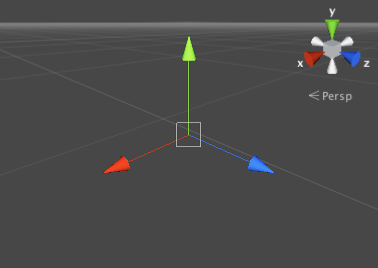
\includegraphics{{Figures/Section3_CoordinateSystem.png}}
	\caption{Coordinate system in Unity}
	\label{fig: Coordinate unity}
\end{figure}\\
Screen coordinate system is bottom-up: (0,0) at bottom-left corner and (pixelWidth-1,pixelHeight-1) at right-top; x axis is positive right and y is positive up. The z position is in world units from the camera.\\
Viewport coordinate system is normalized and relative to the camera, so the bottom-left point is (0,0), the top-right is (1,1). The z position is in world units from the camera.\\
Finally UI coordinate system is top-down: the y coordinate varies from zero at the top edge of the window to a maximum at the bottom edge of the window. The upper-left point is (0,0); the bottom-right is (1,1).\\
There are many functions to convert between all these different coordinate systems
\subsection{Basic principle in scene}
\subsection{Basic knowledge of script}

\dots
